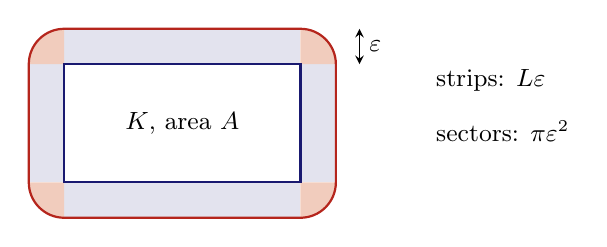
\begin{tikzpicture}[x=1cm,y=1cm,font=\small,>=stealth]
\fill[MidnightBlue!12] (0,-.45) rectangle (3,0);
\fill[MidnightBlue!12] (0,1.5) rectangle (3,1.95);
\fill[MidnightBlue!12] (-.45,0) rectangle (0,1.5);
\fill[MidnightBlue!12] (3,0) rectangle (3.45,1.5);
\fill[BrickRed!18] (0,0)--(-.45,0) arc[start angle=180,end angle=270,radius=.45]--cycle;
\fill[BrickRed!18] (3,0)--(3,-.45) arc[start angle=270,end angle=360,radius=.45]--cycle;
\fill[BrickRed!18] (3,1.5)--(3.45,1.5) arc[start angle=0,end angle=90,radius=.45]--cycle;
\fill[BrickRed!18] (0,1.5)--(0,1.95) arc[start angle=90,end angle=180,radius=.45]--cycle;
\draw[MidnightBlue,thick] (0,0) rectangle (3,1.5);
\draw[BrickRed,thick,rounded corners=12.8pt] (-.45,-.45) rectangle (3.45,1.95);
\node at (1.5,.75) {$K$, area $A$};
\draw[<->] (3.75,1.5)--node[right] {$\varepsilon$}(3.75,1.95);
\node[anchor=west] at (4.6,1.3) {strips: $L\varepsilon$};
\node[anchor=west] at (4.6,.65) {sectors: $\pi\varepsilon^2$};
\end{tikzpicture}
